\section{启动Ray搭建集群环境}

\subsection{启动Ray head节点}
通过命令行运行以下代码启动Ray的head节点:
\lstset{language=Bash}
\begin{lstlisting}
    ray start --head
\end{lstlisting}

屏幕会正常输出以下内容:
\lstset{language=Bash, breaklines, columns=flexible}
\begin{lstlisting}
(base) C:\Users\刘铭\Downloads>ray start --head
Local node IP: 192.168.1.118
2021-02-23 16:55:53,531 INFO services.py:1171 -- View the Ray dashboard at http://localhost:8265

--------------------
Ray runtime started.
--------------------

Next steps
  To connect to this Ray runtime from another node, run
    ray start --address='192.168.1.118:6379' --redis-password='5241590000000000'

  Alternatively, use the following Python code:
    import ray
    ray.init(address='auto', _redis_password='5241590000000000')

  If connection fails, check your firewall settings and network configuration.

  To terminate the Ray runtime, run
    ray stop
\end{lstlisting}

\subsection{向集群添加子节点}
根据head节点启动后的提示,在另外几台计算机中,输入以下命令:
\lstset{language=Bash}
\begin{lstlisting}
    ray start --address='192.168.1.118:6379' --redis-password='5241590000000000'
\end{lstlisting}

如果该节点ray正常安装,并且该节点能够与head节点正常通信,屏幕会输出以下内容:
\lstset{language=Bash, breaklines, columns=flexible}
\begin{lstlisting}
Local node IP: 192.168.1.134

--------------------
Ray runtime started.
--------------------

To terminate the Ray runtime, run
  ray stop
\end{lstlisting}

在添加子节点时,可指定一台计算机有几个CPU和GPU,用命令$ --num-cpus=10 \quad --num-gpus=1 $表示,更多Ray配置信息可查看\href{https://docs.ray.io/en/master/configure.html#configuring-ray}{官方页面}。

若出现以下错误信息,则是因为网络IP无法访问:
\lstset{language=Bash, breaklines, columns=flexible}
\begin{lstlisting}
Unable to connect to Redis. If the Redis instance is on a different machine, check that your firewall is configured properly.--port
\end{lstlisting}

可通过$ ping $工具进行检测,测试数据包能否透过IP协议到达head节点主机,如图\ref{Ping工具检测网络连接}所示。
\begin{figure}[h]
    \centering
    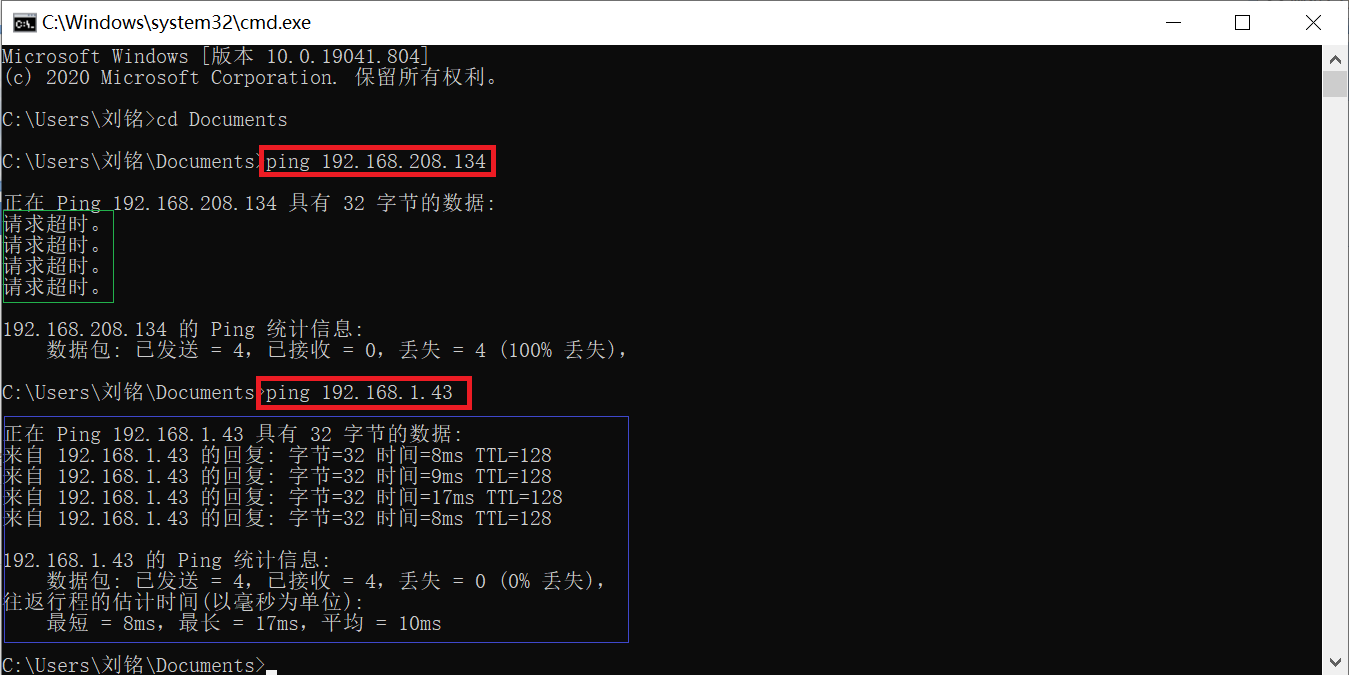
\includegraphics[width=1.0\textwidth]{ping.png}
    \caption{Ping工具检测网络连接}
    \label{Ping工具检测网络连接}
\end{figure}

\subsection{在Ray集群上运行Ray程序}
要在分布式Ray集群环境下运行程序,需要在与节点之一的机器上执行程序,并且在其他每台计算机中安装好相同的运行环境。
\subsubsection{初始化Ray}
在程序/代码中,您必须调用ray.init并将address参数添加到中ray.init,使得Ray连接到现有群集。例如:
\lstset{language=Bash, breaklines, columns=flexible}
\begin{lstlisting}
    ray.init(address="auto")
\end{lstlisting}

若要验证已成功加入集群的节点数量,可以运行以下代码:
\lstset{language=python, breaklines, columns=flexible, numbers=left}
\begin{lstlisting}
import ray
import time

@ray.remote
def f():
    time.sleep(0.01)
    return ray.services.get_node_ip_address()

set(ray.get([f.remote() for _ in range(1000)]))
\end{lstlisting}

\subsubsection{在代码中调用ray的API}
Ray为方便用户更好的使用,提供了大量API供用户使用,如$ ray.init $、$ ray.is\_initialized $、$ ray.remote $、$ ray.get $、$ ray.method $等等,具体使用方式见\href{https://docs.ray.io/en/master/package-ref.html#}{Ray官方API文档}。